\documentclass{article}
\usepackage{geometry}
\usepackage{indentfirst}
\usepackage{float}
\usepackage{graphicx}
\usepackage{multirow}

\author{
    Jiewen Hai\\
    3035456935
    \and
    Jiaqi Deng\\
    3035419509
} 

\title{COMP7506 Smart phone apps development\\Guardian}

\date{}
\begin{document} 
\maketitle

\setcounter{tocdepth}{2}
\tableofcontents

\section{Background}
Nowadays, telephone deception has become more and more common and frequent. It already has grabbed the public attention. To avoid the public from being deceived by telephone deception, this project aims to arise people’s awareness of internet security by providing a mobile application which can show newest pop-up warning message to alert users and help users gain more information about the incoming calls. Additionally, the application enables users to choose alert level, to block unwanted numbers and to manage the block-list.

\section{Additional Features}
\subsection{Alert Level}
While users have an unknown incoming call, a pop-up warning image might show on top of the interface of incoming call according to the alert level.

There are 2 levels of alert. One is to alert every call that is not from the phone book. The other is only showing the alert image when the incoming call is tagged as high frequency number. The default mode of alert function is the all unknown call. Users must choose one of modes to execute the alert action. The default one is to alert all unknown calls.

\subsection{Block calls}
The application provides block function. Blocked numbers will be automatically hung up by the application. To execute the function, application needs to gain the authorization from users when the application is downloaded and started in the first time.

Block mode has the same 2 levels like alert. One is to block every unknown call and the other is only blocking the high frequency call. The difference between alert and block is that block mode can be turned off which means that users do not have to block any calls. While the block mode is turned on, one of the mode must be chosen. The default one is to block all unknown call

In this scenario, user unwanted numbers will not directly reach to user and user can browser and manage the blocked number in the block-list inside the application.

\begin{figure}[H]
    \centering 
    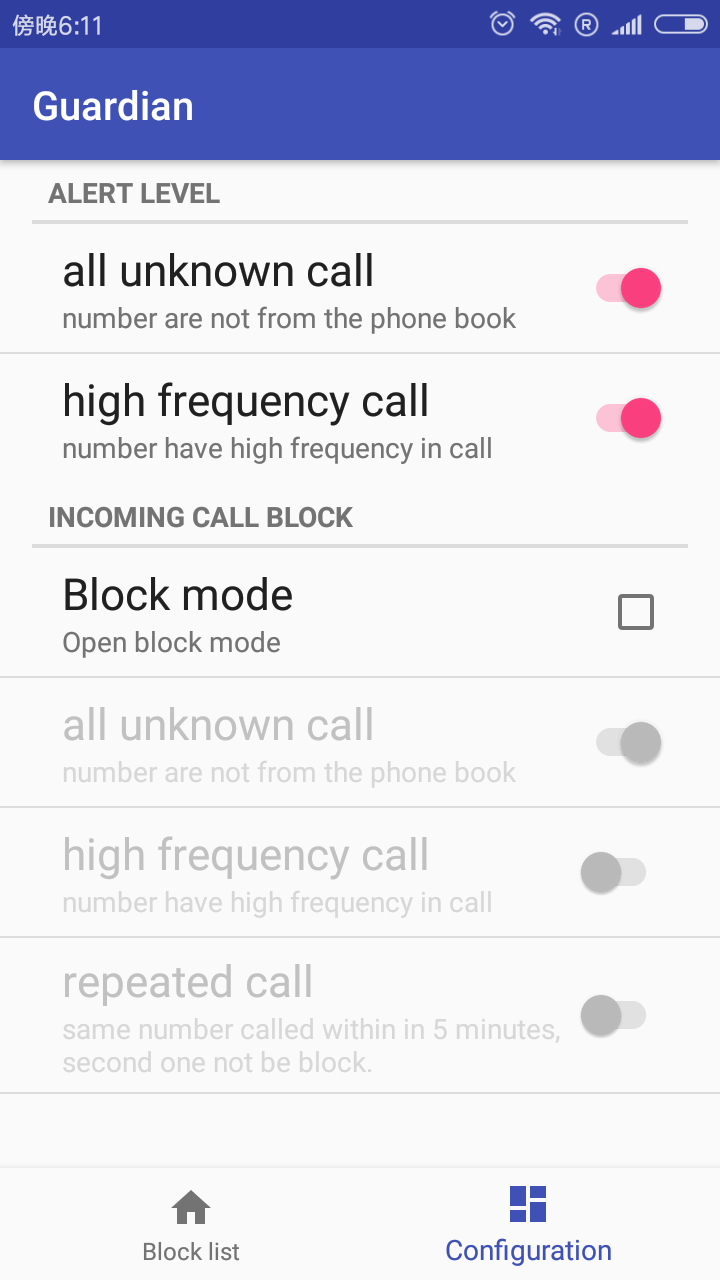
\includegraphics[width=0.418\textwidth]{images/config.jpg}
    \caption{Configuration page}
    \label{image_config}
\end{figure}

\subsubsection{Repeated calls}
Moreover, block mode has an additional feature, repeated call. The feature of repeated call is based on the block mode. This feature only works when a number has been blocked. When user turn on this feature, if a blocked number call twice in 5 minutes, the second one in call will not be block and can reach out to the user. The default mode is in close status.

\subsection{Tag/Add unknown calls}
Apart from alerting and blocking umbers, the application also provides some management functions for users to manage the unknown in-coming calls, including add and tag.

After opening the application, it shows the recent calls interface which contains all incoming calls with time format. Users can tag an unknown call by choosing one of types shown on screen including promotion, delivery and fraud. This function helps application learn the unknown phone numbers inside its database. Additionally, users can add an unknown number into the phone book in the application by touching the . 

The interface of tagging /adding unknown calls is shown below:
\begin{figure}[H]
    \centering 
    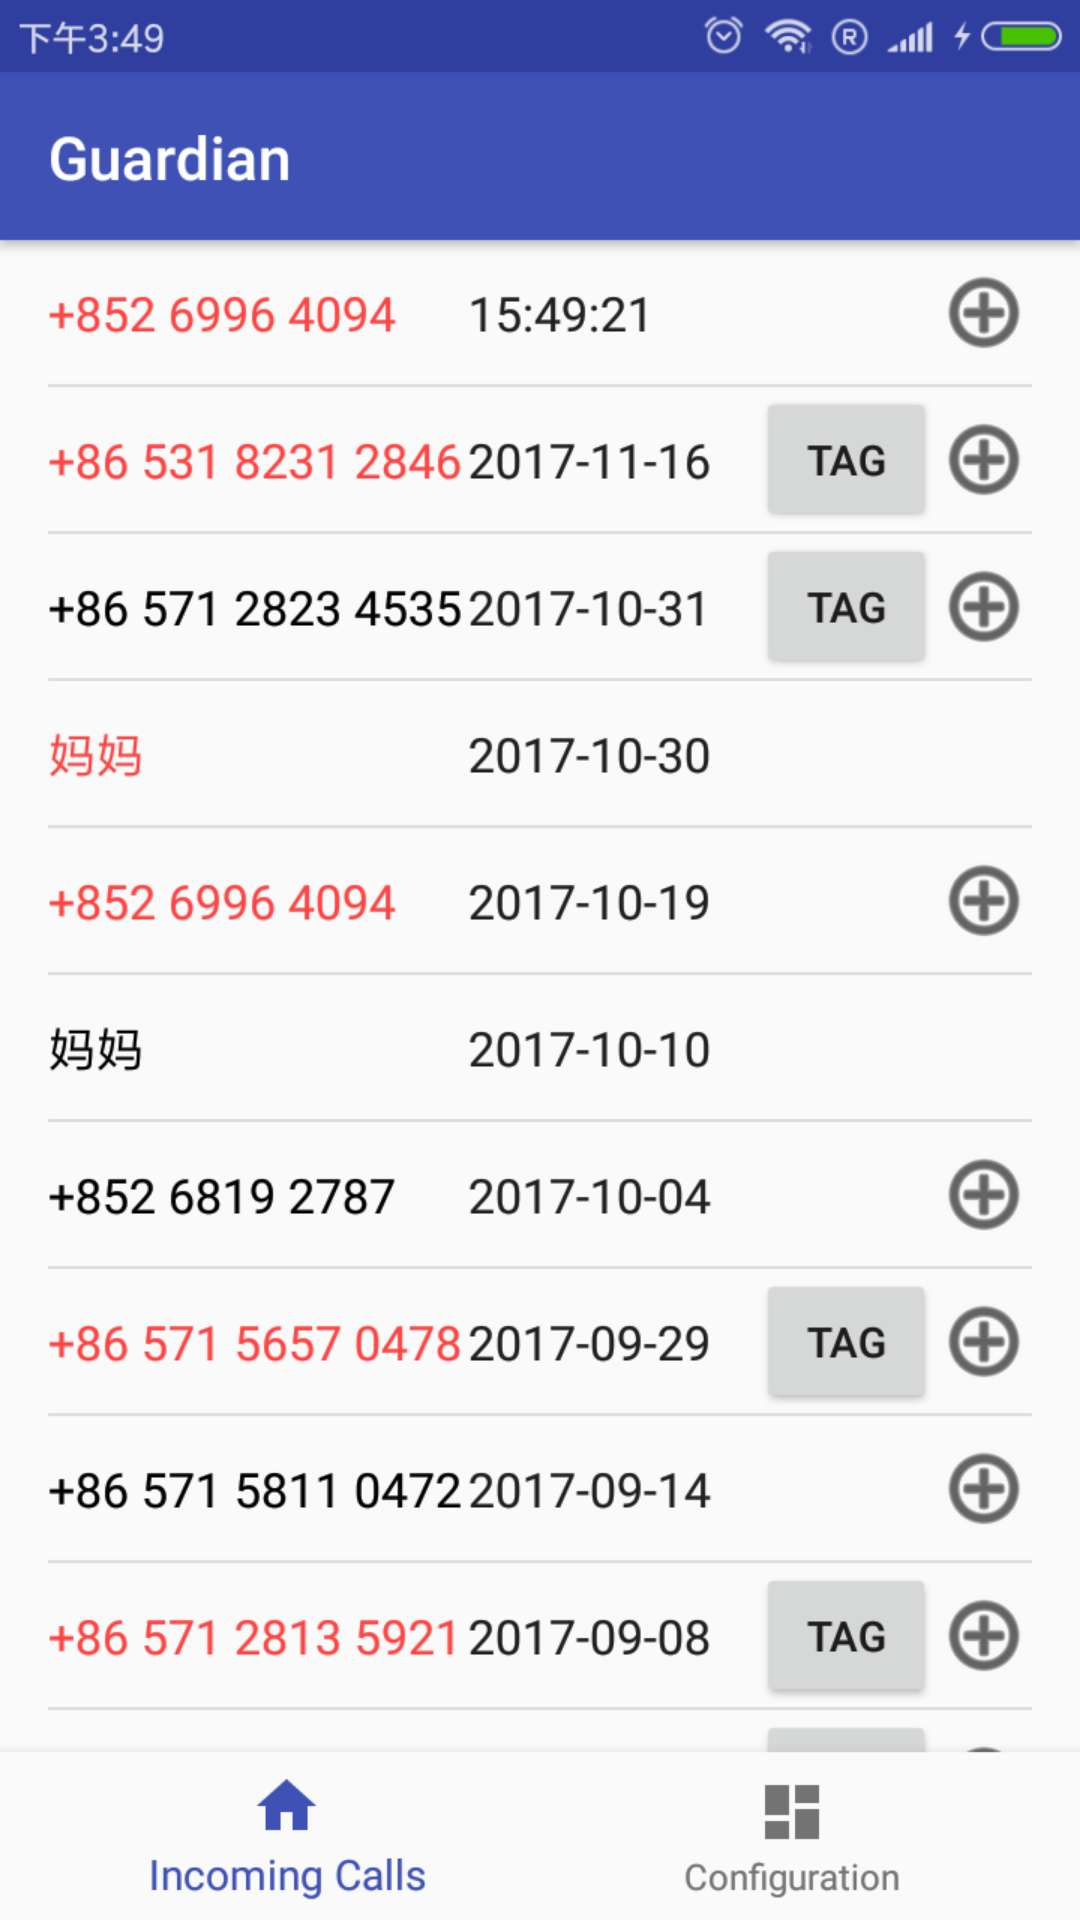
\includegraphics[width=0.418\textwidth]{images/calls.jpg}
    \caption{Incoming calls page}
    \label{image_calls}
\end{figure}

\section{Usage}

\section{Technology}
This part briefly introduces some core technologies used in the program. The project is composed of three modules, \textbf{client}, \textbf{common} and \textbf{server}.

\begin{itemize}
    \item \textbf{client} is responsible for interacting with user and visualizing the data.
    \item \textbf{server} collects the data from the client and persist them into database.
    \item \textbf{common} define a TCP protocol between Client and Server allowing more performance than HTTP protocol.
\end{itemize}

\subsection{Client}
The client is the most complex module in this project. from perspective of functionality, we have three major demand, blocking, config and tag. User need a screen to browse all incoming calls to tag them as malicious calls. And another screen is necessary to configure the metadata of block and alert. We need to upload tag information to server and download them according to phone number to alert user or block incoming phone.

\subsubsection{MainActivity}
\textbf{MainActivity} has two major tasks, which are requesting permission and managing two functional components \textbf{BlockFragment} and \textbf{ConfigFragment} respectively. Before instantiate the actual fragment, it would request all permission from user, and check whether they are all granted. If not, the application would close itself.

The \textbf{MainActivity} utilize \textbf{ViewPager} and \textbf{BottomNavigationView} to switch two fragments. But we do not wish user drag fragments with touch, thus, a \textbf{NoScrollViewPager} is introduced, which is subclass of \textbf{ViewPager}. The drag functionality of \textbf{ViewPager} is disabled by override the touch event method.

\subsubsection{BlockFragment}
\textbf{BlockFragment} utilize \textbf{LoaderManager} to load data asynchronously. A \textbf{CursorLoader} is created to load data from \textbf{CallLog}. Process the data, put them into a \textbf{List} and pass them into a \textbf{BlockAdapter}.

I adopt \textbf{ViewHolder} pattern in the adapter. I only instantiate views and locate them once, and put the references into tag.  Next time, we just need to bind data to that item. We need to fetch data from flash to update the item, thus, a asynchronous task is necessary. The \textbf{BlockAdapter.UpdateView} task is instantiate with a view holder and a data item. Once it finish the task, it will update the UI. However, two task might update same view holder. In order to counter it, \textbf{optimistic concurrency control} is implemented. We add a version field for every view holder, and check the version before update automatically. Once the update is finished, we check whether the version is same. Abort the task if the version is updated. 

\subsubsection{ConfigFragment}
This section is very simple, we just utilized \textbf{PreferenceFragmentCompat} to manage all shared preference. A ConfigHolder is created as a proxy to access all configuration data.

\subsubsection{TagDatabase}
\textbf{Room} \cite{room} is ORM framework, which facilitate our development drastically. Only one table is created, which is \textbf{TagCommand}. This table maintains all $(phone, tag)$ pair and has filed $uploaded$ to record this tuple is whether uploaded or not. We access the data through \textbf{TagDao}. The \textbf{Room} framework would translate all of this annotation into SQL language.

\subsubsection{UploadService}
A \textbf{BlockingQueue} is instantiated in \textbf{UploadService}. And we got a \textbf{Thread} to pull item from that. Once the item is fetched, check whether it is the end signal. If it is, just end the thread, otherwise, check database and upload tag information. Every time we insert data or enter resume \textbf{MainActivity}, we also send a signal into that queue to notify update.

Since the upload action is asynchronous. I implement a blocking counter to check whether the action is finished. If the connection is broken, or uploading failed, the counter is reset, and terminate this action.

\subsubsection{PhoneBlocker}
PhoneBlocker is a \textbf{BroadcastReceiver}, which intercept all incoming calls. The PhoneBlocker will read the data from database, preference and network, then decided whether alert, block or just let it go. Cause Android hide the telephone management api, we need utilize \textbf{Reflect} api to get the method. So that, we could block the call. And it also might start a warning activity. 

\subsubsection{AlertActivity}
\textbf{AlertActivity} will popup when we need to alert the user. It use \textbf{Volley}'s \textbf{NetworkImageView} \cite{volley}to download the image. And poll data from sever to render a tag pie chart using \textbf{HelloCharts}. But one thing is need to be taken care of. We must cover the incoming call screen. Thus, we send a delayed message to a \textbf{Handler}. It would start the activity again and render the graphics.
\subsection{Protocol}
We adopt \textbf{Netty} \cite{netty} framework to implement protocol over \textbf{TCP} layer. And `RxJava` is acted as middle-ware to propagate data. We only defined two pair of operation to transfer data. The number within parentheses is number of bytes.

\begin{itemize}
    
    \item Tag: \textbf{TagRequest} and \textbf{TagResponse}. This protocol upload tag information to server.

    \begin{table}[!hbp]
        \centering
        \begin{tabular}{|c|c|c|c|c|c|}
        \hline
        type(1) & length(2) & seq no.(4) & phone len.(1) & phone no.(LN) & tag(LT)\\
        \hline
        \end{tabular}
        \caption{Tag Request}
    \end{table} 

    \begin{table}[!hbp]
        \centering
        \begin{tabular}{|c|c|c|}
        \hline
        type(1) & length(2) & seq no.(4)\\
        \hline
        \end{tabular}
        \caption{Tag Response}
    \end{table} 

    \item Inquiry: \textbf{InquiryRequest} and \textbf{InquiryResponse}. Thi protocol send a phone number to server and retrieve all tag information of this number.

    \begin{table}[!hbp]
        \centering
        \begin{tabular}{|c|c|c|c|}
        \hline
        type(1) & length(2) & seq no.(4) & phone no.(LN)\\
        \hline
        \end{tabular}
        \caption{Inquiry Request}
    \end{table} 

    \begin{table}[!hbp]
        \centering
        \begin{tabular}{|c|c|c|c|c|c|c|}
        \hline
        type(1) & length(2) & seq no.(4) & size.(1) & $len_1$ & $tag_1$(LT) & $time_1$(4)  \\
        \hline
         ... & $len_{size}$ & $tag_{size}$(LT) & $time_{size}$(4) & & &\\
        \hline
        \end{tabular}
        \caption{Inquiry Response}
    \end{table} 

\end{itemize}

\textbf{MessageDecoder} would convert the binary stream into object. It would invoke \textbf{MessageFactory} to instantiate \textbf{Message} object, and decode them. \textbf{MessageHandler} push this message to the processor flow. And the downstream could subscribe this flow. All request message hold \textbf{ChannelHandlerContext}, which allow the downstream write back. \textbf{MessageEncoder} encode the response into binary stream by invoking encode method.

\subsection{Server}
\textbf{Server} is the most simple module. It utilize \textbf{Spring} \cite{spring} framework to assemble components.

\textbf{CallService} implement two simple method. \textbf{Tag} would invoke the stored function defined in database, this stored function would guarantee the atomicity of tag transaction in concurrent scenario. \textbf{Inquiry} is just a select, it utilize \textbf{JDBCTemplate} to de-serialize data.

In order to achieve atomicity in database, we utilized a \textbf{pg\_advisory\_xact\_lock} in postgresql \cite{pg}. This lock will maintain until the transaction is perform. This lock intend to handle the \textbf{Phantom Read} issue, thus, we only need to acquire this lock when we need to insert new row. When we only need to update the total times of tag, we rely on postgresql's \textbf{Multi-Version Concurrency Control}.

\bibliographystyle{plain}
\bibliography{reference}
\end{document}